\section{Experiments} \label{sec:impl}

We have implemented an interpreter for the language in
Figure~\ref{fig:syntax} based on the probabilistic polyhedra powerset
domain as well the simpler probabilistic domains constructed from the
interval and octagon base domains. The manipulations of base domain
regions are done using the Parma Polyhedra Library
\cite{parma} (ppl-0.11.2). Counting calculations are done using the LattE
\cite{latte} tool (LattE macchiato 1.2-mk-0.9.3) in the case of
polyhedra and octagons. The trivial counting
calculation for the interval domain we implemented ourselves as part
of the abstract interpreter, which itself is written in OCaml (3.12.0).  While
many of the abstract operations distribute over the set of
probabilistic regions and thus could be parallelized, our
implementation is currently single-threaded.

% Lacking off-loaded computation, our current implementation can also be
% improved in a variety of ways as optimization was not an important
% consideration during development. Parallelization in particular could
% have great impact. The powerset domains operations are largely
% operations on component probabilistic polyhedra, which can naturally
% be done in parallel. The task of picking the optimal merging order
% discussed above can also be performed in parallel.

This section presents an experimental evaluation of
our implementation on several benchmark programs.  Overall, the
use of the octagonal and polyhedral domains results in running times
ranging from a few seconds to a few minutes. Compared to 
enumeration-based approaches to probabilistic computation, using
probabilistic polyhedra improves running times by up to 1--2 orders of
magnitude.  Intervals do even better, with running times ranging from
tens to hundreds of milliseconds, constituting an additional 1--2
orders of magnitude improvement.  For our particular experiments,
exact precision is reached by all 
domains if the bound on the number of regions is sufficiently large.

Our experiments
were conducted on a Mac Pro with two 2.26 GHz quad-core Xeon
processors using 16 GB of RAM and running OS X v10.6.7.  

\subsection{Benchmark Programs}
\label{sec:benchmarks}

We applied our implementation to several queries. The timings measure,
for each query, the construction of a pre-belief, the probabilistic
evaluation of a query, and finally a policy check over all secret
variables. We describe each query here, and show the complete source
code, pre-belief, and further details in
Appendix~\ref{appendix:queries}.

\paragraph{Birthday} We benchmark the birthday queries described in
Section~\ref{sec:overview}:
\begin{itemize}
\item{\textbf{bday 1}} The first birthday query
  (Example~\ref{ex:bday}).
%\item{\textbf{bday (large) 1+2}} After two birthday queries, the
%  second of which has ``today'' set to one day after the first query.
\item{\textbf{bday 1+2+special}} The sequence of the first two
  birthday queries (Example~\ref{ex:bday} and then the same code, but
  with $\mathit{today}$ increased by 1) followed by the special
  birthday query (Example~\ref{ex:specyear}).  Below we refer to
  this benchmark as the \emph{birthday query sequence}.
\end{itemize}
We consider \emph{small} and \emph{large} variants of these two
queries: the former assumes the birth year ranges from 1956 to 1992,
while the latter uses the range 1910 to 2010.

\paragraph{Pizza} This query evaluates whether a user might be 
interested in a local pizza parlor. To do this, the code checks
whether the user's location is within a certain square area and
whether they match an age or current education criteria most
associated with pizza-eating habits (18-28 year old or currently
undergrad or above). The modeled secret variables thus include: the
user's birth year, the level of school currently being attended, and
their address latitude and longitude (scaled by $10^6$ and represented
as an integer). The last two variables have large magnitudes.  The
true values used in the benchmark were $39003178$ and $−76958199$ for
latitude and longitude, respectively.

\paragraph{Photo} This query is a direct encoding of a real
targeted advertisement that Facebook includes on their information
page \cite{wedding-case-study}. The query itself checks whether the
user is female, engaged, and is in a certain age range, indicative of interest
in (wedding) photography service. There are three secret variables in this
example: gender, relationship status, and birth year.

\paragraph{Travel} This query is another adaptation of a
Facebook advertisement case study \cite{visitbritain-case-study},
based on a campaign run by a tourism agency. The aim of the query is
to determine whether the user lives in one of several relevant
countries, speaks English, is over the age of 21, and has completed a high
level of education. The secret variables thus include four dimensions:
the user's country of residence, birth year, highest level
of completed education, and primary language.

\paragraph{Is Target Close, Who is Closer} These queries were designed to
demonstrate the need for relational abstractions. They perform simple
(Manhattan) distance calculations over points defined by 2D
coordinates. \textbf{Is Target Close} checks whether an unknown point is
within some distance of a given point and \textbf{Who is Closer}
determines which of two unknown points is closer to a given point. The
nature of these queries is further discussed in \sref{sec:relational}
and their full specification is shown in
Appendix~\ref{sec-appendix-relational}.

\subsection{Comparison to Enumeration} \label{sec:enum}

\begin{figure}[t!]
\centering
\begin{tabular}{c}
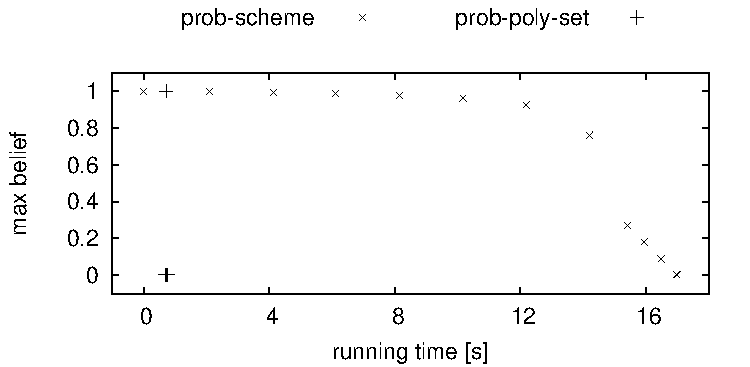
\includegraphics[width=9cm]{figures/plot_bday.pdf} \\
(a) birthday query \textbf{bday 1 (small)} \\
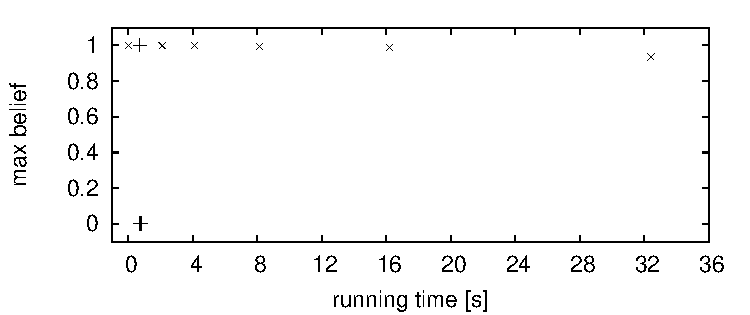
\includegraphics[width=9cm]{figures/plot_bday_large.pdf} \\
(b) birthday query, larger state space - \textbf{bday 1 (large)} \\
%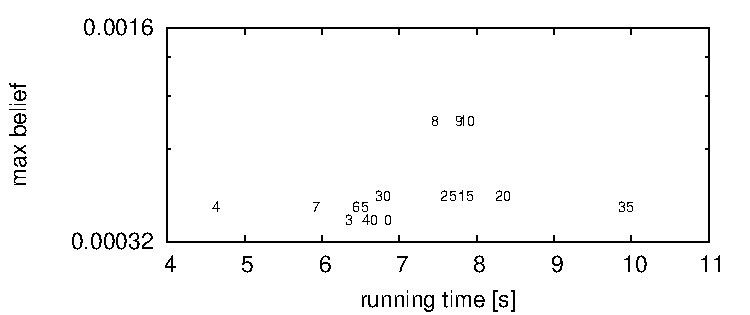
\includegraphics[width=9cm]{figures/plot_bday_seq.pdf} \\
%(c) special year query (\eref{ex:specyear})
\end{tabular}
\caption{Query evaluation comparison}
\label{fig:plots_bday}
\end{figure}

\fref{fig:plots_bday}(a) illustrates the result of running the
\textbf{bday 1 (small)} query using our implementation and one using
Probabilistic Scheme~\cite{radul07probscheme}, which is capable of
sound probability estimation after partial enumeration.  Each $\times$
plots prob-scheme's maximum probability value (the y axis)---that is,
the probability it assigns to the most likely secret state---when
given a varying amount of time for sampling (the x axis).  We can see
the precision improves steadily until it reaches the exact value of
1/259 at around 17 seconds. Each $+$ plots our implementation's
maximum probability value when given an increasing number of
probabilistic polyhedra; with a polyhedral bound of 2 (or more), we
obtain the exact value in less than one second. The timing
measurements are taken to be the medians of 20 runs.

The advantage of our approach is more evident in
\fref{fig:plots_bday}(b) where we use the same program but allow
$\var{byear}$ to span 1910 to 2010 rather than 1956 to 1992 (this is
\textbf{bday 1 (large)}).  In this case prob-scheme makes little
progress even after a minute. Our approach, however, is unaffected by
this larger state space and produces the exact maximum belief in less
than one second when using only 2 probabilistic
polyhedra.

We can push the advantage much further with the use of the simpler
interval domain which can compute the exact probabilities in both the
smaller and larger birthday examples, using only 2 intervals, in
around 0.008 seconds. These benchmarks can be seen in
Figure~\ref{fig:bench_domains_bday}, discussed shortly.

\subsection{Performance analysis}
\label{sec:perf-analysis}

Figures~\ref{fig:bench_domains_bday}-\ref{fig:bench_domains_travel}
summarize the performance results for all the benchmarks programs and
for each of the three base domains. The raw data producing these
figures are found in Table~\ref{fig:bench_table} in the appendix. The
bottom graph of each figure zooms in on the results for the interval
domain which can also be seen in the upper graphs.

The timing benchmarks in the figures are based on 20 runs, the median
of which is denoted by one of three symbols: a box, a diamond, and a
pentagon for the interval, octagon, and polyhedron domains,
respectively. The symbols are scaled based on the precision in max
probability, relative to exact, the analysis achieves; a tiny dot
signifies exact probability and increasing symbol size signifies
worsening precision. Note, however, that the sizes of the symbols are
\emph{not} proportional to precision. The vertical gray boxes range from
the 1st to 3rd quartiles of the samples taken while the vertical lines
outside of these boxes represent the full extent of the samples.

We discuss the performance and precision aspects of these results in turn.

\begin{figure}[t!]
\scriptsize
\centering
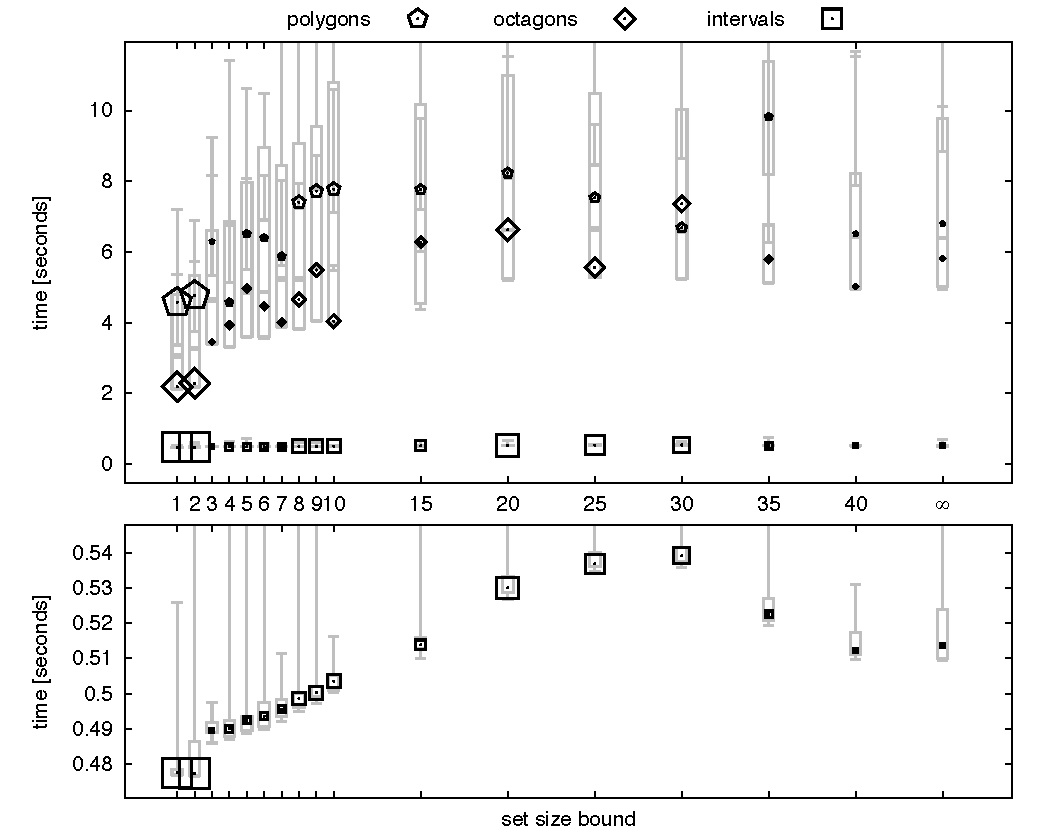
\includegraphics[width=12.5cm]{figures/plot_domains_bday.pdf} \\
\caption{birthday query sequence benchmarks}
\label{fig:bench_domains_bday}
\end{figure}

\begin{figure}[t!]
\scriptsize
\centering
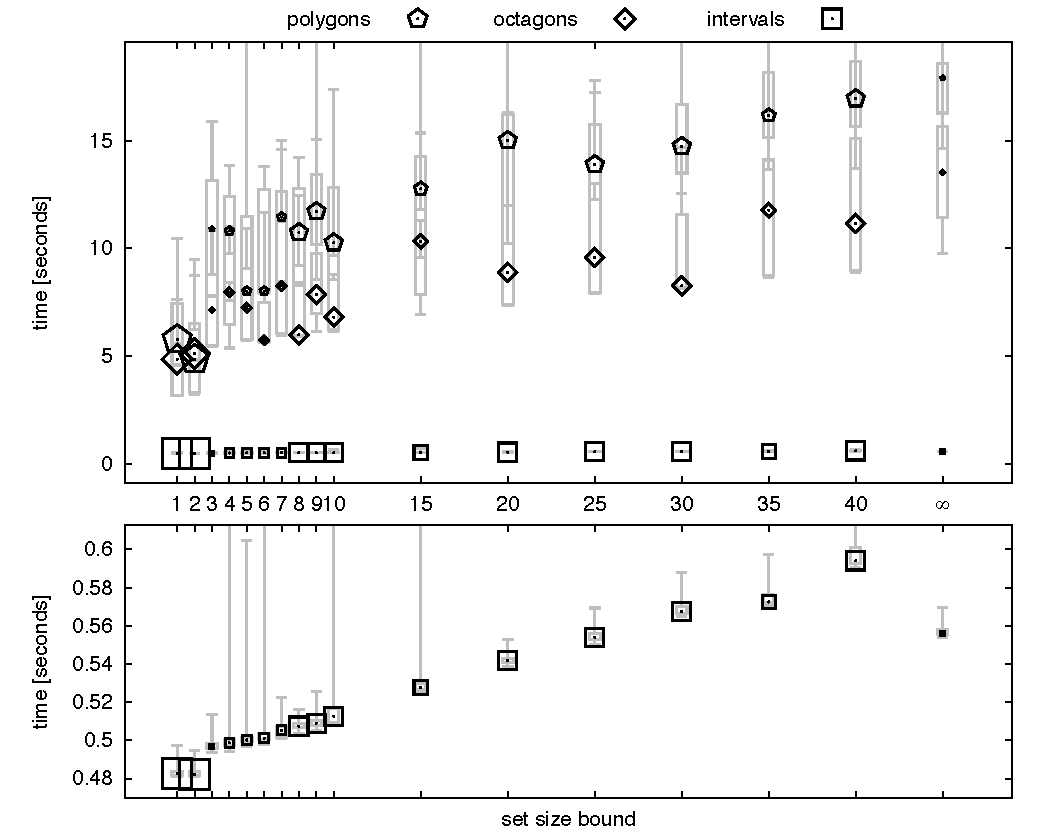
\includegraphics[width=12.5cm]{figures/plot_domains_bday_large.pdf} \\
\caption{birthday (large) query sequence benchmarks}
\label{fig:bench_domains_bday_large}
\end{figure}

%\paragraph{Special Birthday Queries}
%Figures~\ref{fig:bench_domains_bday} and
%\ref{fig:bench_domains_bday_large} show the result of our
%implementations assessing the special query
%(Example~\ref{ex:specyear}) following two birthday queries, with
%either the smaller or larger initial belief state-space respectively
%Relative to the simpler birthday queries (Figure~\ref{fig:plots_bday}
%(a) and (b)), the plot demonstrates that more complex queries,
%specifically ones with many disjunctions in their conditionals, not
%only slow our approach, but also reduce the precision of the maximum
%probability value. The first, smaller state-space, example requires 36
%polyhedra for exact calculations though as little as 3 produce exact
%probabilities. Note that the precision does not increase monotonically
%with the number of polyhedra---in some cases more polyhedra leads to a
%less precise result. We conjecture that the occasional worsening of
%the precision with increase in the number of allowable polyhedra is
%due to an overly simple means of deciding which polyhedra to merge
%when performing abstract simplification.
%
%Using the interval base domain we can asses the special birthday query
%exactly (assuming a sufficiently large bound on the number of
%intervals) in around 0.47 seconds, as compared to around 21 seconds
%for the polyhedron base domain (see Table~\ref{fig:bench_table}).

\begin{figure}[t!]
\scriptsize
\centering
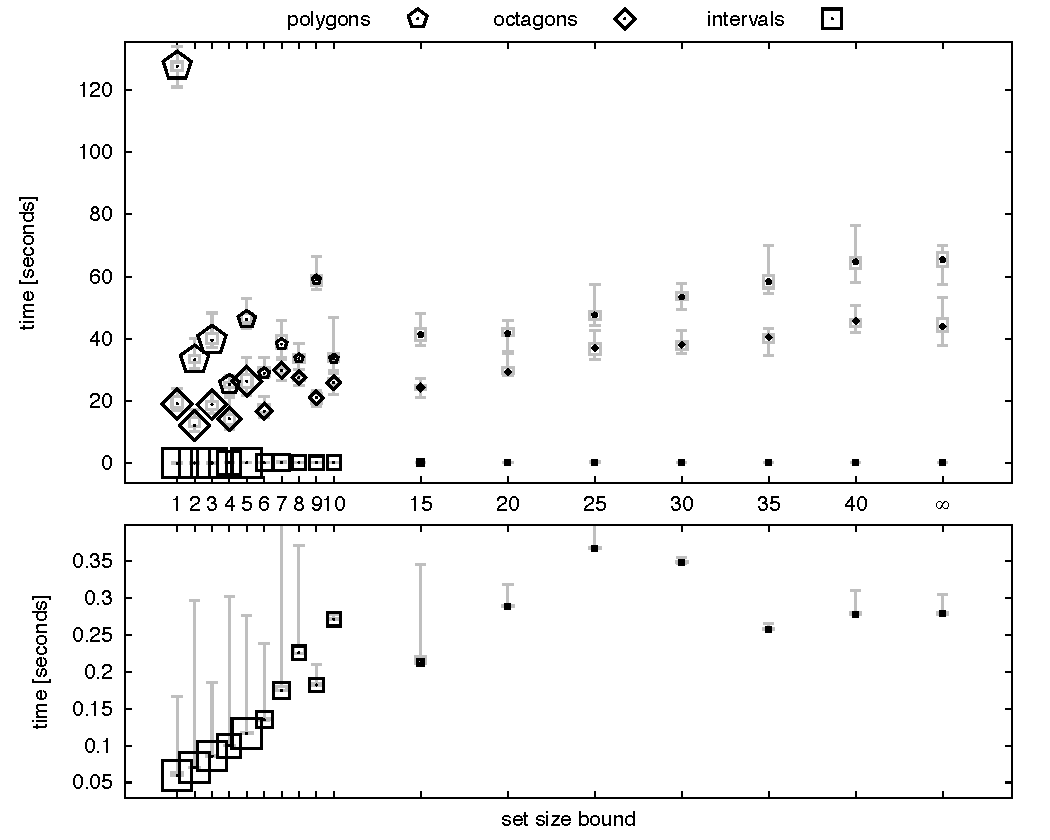
\includegraphics[width=12.5cm]{figures/plot_domains_pizza.pdf} \\
\caption{pizza query benchmarks}
\label{fig:bench_domains_pizza}
\end{figure}

\begin{figure}[t!]
\scriptsize
\centering
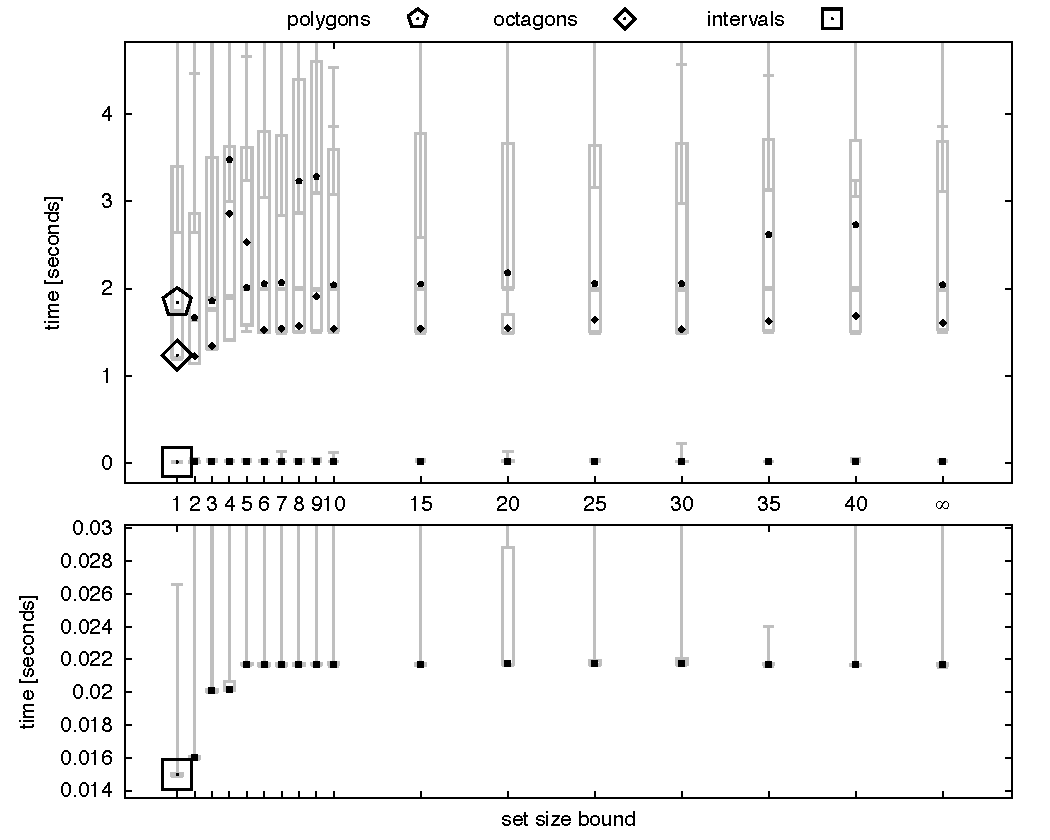
\includegraphics[width=12.5cm]{figures/plot_domains_photo.pdf} \\
\caption{photo query benchmarks}
\label{fig:bench_domains_photo}
\end{figure}

\begin{figure}[t!]
\scriptsize
\centering
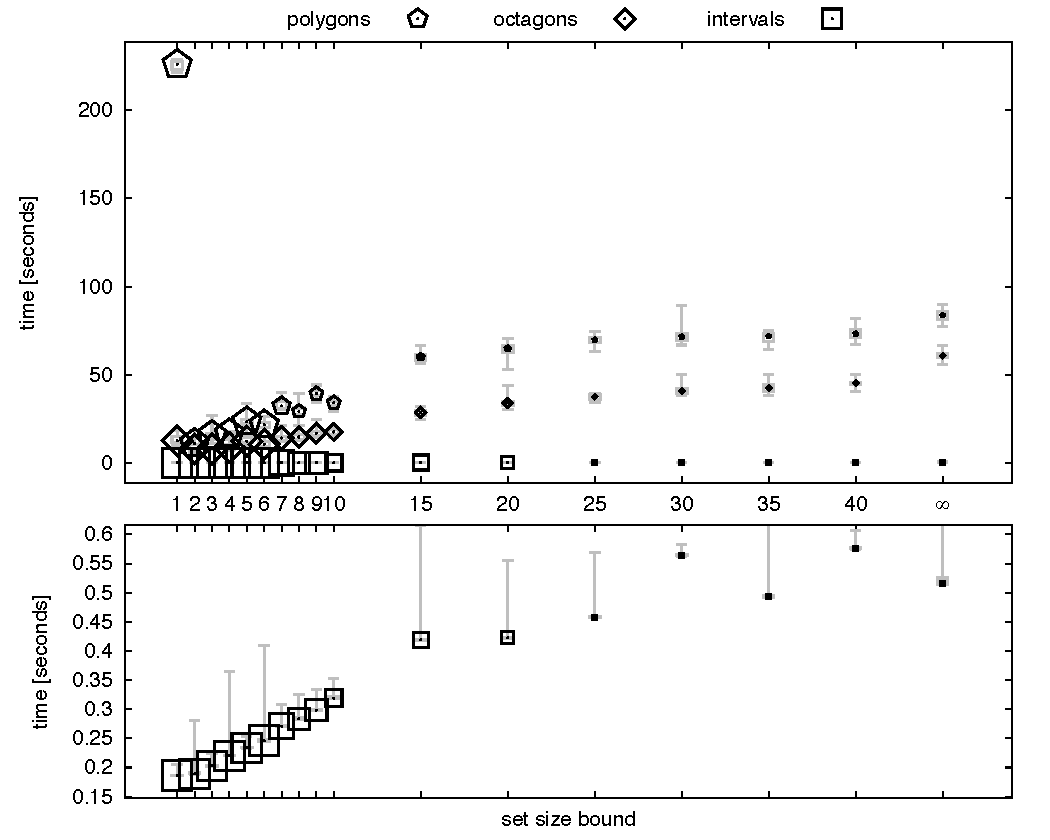
\includegraphics[width=12.5cm]{figures/plot_domains_travel.pdf} \\
\caption{travel query benchmarks}
\label{fig:bench_domains_travel}
\end{figure}

\begin{figure}[t!]
\scriptsize
\centering
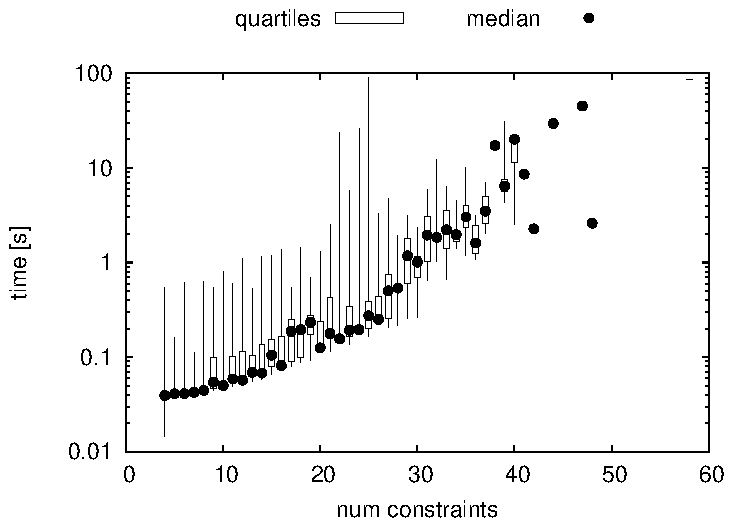
\includegraphics[width=8.5cm]{figures/plot_latte.pdf} \\
\caption{LattE benchmarks}
\label{fig:bench_latte}
\end{figure}

\paragraph*{Performance.}
Overall, the use of the octagonal base domain results in slightly
improved performance over the polyhedral base domain. The interval
domain, however, is much faster than both due to the simpler counting
and base domain operations.  Though the performance gains from the use
of octagons are meager, we note that it is likely they can be greatly
improved by implementing a octagon-specialized counting method instead
of using the general polyhedron counting tool (LattE).

As the number of base domain regions increases, the running time
generally increases, though there are exceptions to this trend.  A
good example can be seen with intervals in
Figure~\ref{fig:bench_domains_bday_large}. Specifically, when there is
no interval set size bound, the analysis takes a less time than with a
bound of 40 (and even produces a more precise answer). In such
situations the additional computational cost of manipulating a larger
number of regions is less than the cost that would have been incurred
by having to merge them to maintain some (large) bound.

In the cases of polyhedron and octagon base domains, the running time
oddities are due to the difficulty of accurately counting points in
complex regions.  We measured that, when evaluating the various
queries in
Figures~\ref{fig:bench_domains_bday}-\ref{fig:bench_domains_travel},
95\% or more of the running time is spent in LattE, performing
counting.  \fref{fig:bench_latte} plots the running time of LattE
against the number of constraints used to define a polyhedron (we used
the polyhedra that arose when evaluating the above queries).  Note
that the y-axis is a log scale, and as such we can see the running
time is super-exponential in the number of constraints.  As such,
overall running time is sensitive to the complexity of the polyhedra
involved, even when they are few in number.  

It turns out that when merging to respect the total bound can result
in complicated shapes which then, unintuitively, increase the running
time.  Two very stark examples of this phenomenon are seen for in the
pizza and travel queries (Figures~\ref{fig:bench_domains_pizza} and
\ref{fig:bench_domains_travel} respectively). With a region bound of
one, the analysis of both these queries takes much longer than with
the bound of two; the large amount of region merging in these
instances resulted in a single, but highly complex region. Using
octagons in both these instances does not result in complex regions
which explains the massive performance improvement. These
observations suggest a great deal of performance improvement can be
gained by simplifying the polyhedra if they become too complex.

%However, due to the uniform region splitting, as we
%discussed in Section~\ref{sec:psimpler}, the octagon-based benchmarks
%are more often than not worse than polyhedron-based ones (as there is
%no uniform region splitting employed there). Future work could
%potentially produce smarter means of splitting simple regions to
%alleviate this problem. 

%Furthermore, the problem of region counting for octagons seems much
%simpler than for polyhedra which suggests performance gains could be
%made using an octagon-restricted counting algorithm.

\paragraph*{Precision.} The figures (and Table~\ref{fig:bench_table}
in the appendix) generally show the trend that the maximum belief
improves (decreases) as the region bound increases, though there are
exceptions.  A good example appears in
Figure~\ref{fig:bench_domains_bday} which depicts the performance of
the birthday query sequence; with a set size bound of 3, the analysis
is able to produce the exact max belief.  Allowing 4 probabilistic
polyhedra (or intervals, octagons), however, does not produce the
exact belief anymore. The same occurs in
Figure~\ref{fig:bench_domains_bday_large} for the larger state space
bday sequence benchmark.

The data also demonstrate that, as expected, the use of polyhedra is
more precise then use of octagons which itself is more precise than
the use of intervals. For the birthday queries, this difference
manifests itself rarely, in particular for the set size bound of 20
and 25 in Figure~\ref{fig:bench_domains_bday}. In the pizza query
benchmarks, polyhedra provide a precision advantage over the other two
domains when the region set size bound is between 5 and 10.  Based on
these sample queries, the precision advantage of using polyhedra or
octagons over intervals seems insignificant. This is due to a general
lack, in these queries, of conditionals that cannot be expressed
exactly when using intervals (or octagons) exactly.
Section~\ref{sec:relational} shows two queries that demonstrate the precision
advantages of polyhedra and octagons more clearly.

\paragraph*{Impact of merge order.} 
Another reason for the the lack of a steady
improvement of precision as the region bound increases is due to order
in which polyhedra are merged.  That is, when simplifying a set of $m$
probabilistic polyhedra to $ n < m $ requires that we iteratively
merge pairs of polyhedra until the bound is reached.  But which pairs
should we use?  The choice impacts precision.  For example, if we have
two largely overlapping polyhedra, we would preserve more precision if
we merge them rather than merging one of them with some other,
non-overlapping one.  We used a deterministic strategy for the
benchmarks in this section, producing identical precision, though some
timing variations.  The question is how well might we have done with a
better strategy?

\begin{figure}[t!]
\scriptsize
\centering
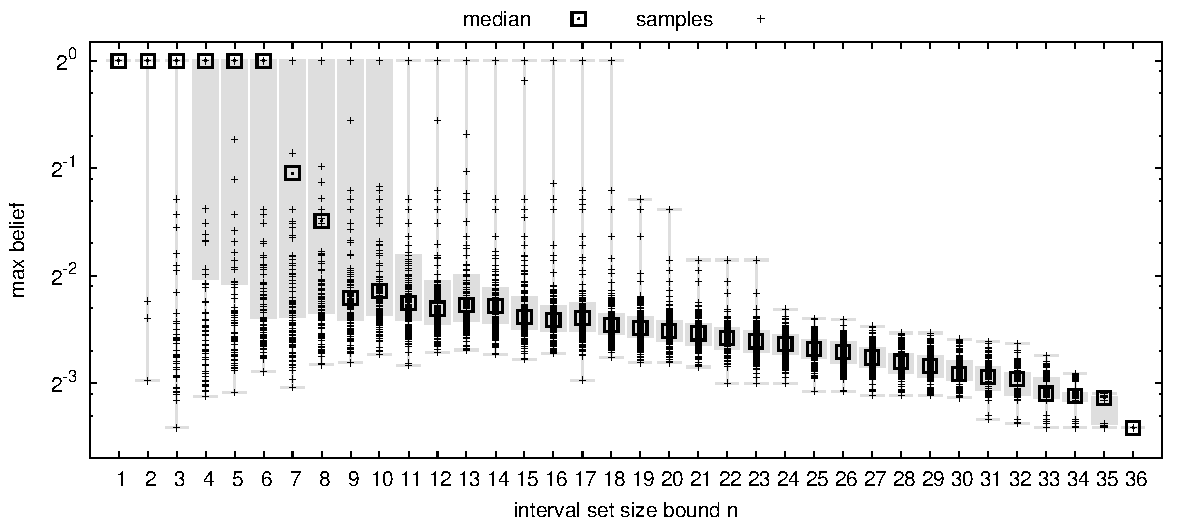
\includegraphics[width=12.5cm]{figures/plot_random_box.pdf} \\
\caption{birthday query sequence precision variation}
\label{fig:random_box}
\end{figure}

To test the precision variation possible due to these arbitrary
choices, we analyzed the birthday query sequence, for each interval
set size bound, but with 200 different random seeds for randomized
merging decisions. The results can be seen in
\fref{fig:random_box}. The median max belief is included, as well as
the lower and upper quartiles (shaded). Note that we did not use the
merging heuristic for the abstract plus operation described in
\sref{sec:powerset} for these measurements (but we do use it in the
results given up to this point).

Naturally there are few arbitrary choices to make when the set size
bound is very low, or very high. In the middle, however, there are
many possibilities. Turning to the figure, we can see the variation
possible is significant except for when the set size bound is at least
36 (at which point there is no merging occurring). For $ n \leq 7 $ it
is more likely than not to conclude max belief is $ 1 $, with $ 1 $
being the median. On the other hand, from as little as $ n = 2 $, it
is possible to do much better, even computing the exact belief (lowest
sample for $ n = 3 $). This itself suggests that our heuristic for the
merging order in abstract plus is useful, as it managed to result in
this exact max belief, against all odds. Also, even though it did not
produce exact beliefs for $ n > 3 $, it did a lot better than the
trivial median one would get by performing merging
randomly. Nevertheless, the merging order is an aspect of the
implementation that has room for improvement, we consider some options
in \sref{sec:future-work}.

From $ n = 8 $, the random merging order starts producing non-trivial
results, on average. Increasing $ n $ further makes it less and less
likely to merge poorly; at $ n = 30 $ for example, no random merge
order out of the 200 samples managed to do terribly, all samples had
belief below $ 0.01 $. Overall, the median max-belief is more or less
monotonically improving as $ n $ increases as one would expect.

An interesting feature of \fref{fig:random_box} is the best max-belief
achieved for each $ n $ (the bottom mark of each column). This
quantity seems to be getting worse from $ n = 3 $ all the way to
around $ n = 14 $ before it starts coming down again. We expect this
is due to two counteracting effects:
\begin{itemize}
\item{} Larger powerset size bound allows for more precise
  representation of distributions, for some merging order.
\item{} It is easier to find a good merging order if there are only a
  few options. For low values of $ n $, most merging orders are
  explored in the 200 samples, hence good orders are found.
\end{itemize}

\subsection{Relational queries} \label{sec:relational}

The examples presented to this point are handled well by the
interval-based abstraction, assuming a sufficient number of intervals
are used.  The simple interval-based abstraction does not work so well
programs that introduce relational constraints on variables.  Such
constraints can arise due to simple distance 
computations, which we would expect to be found in many useful
queries. We provide examples of such computations here (the full
specification of the queries appears in
Appendix~\ref{sec-appendix-relational}). 

Consider an initial belief composed of two pairs of 2-dimensional
coordinates, specifying the location of two objects: $ (x_1,y_1),
(x_2,y_2)$. The \textbf{Is Target Close} query checks
whether the first of the objects is within a specified distance $ d $
from a specified coordinate $ (x,y) $. Distance is measured using
Manhattan distance, that is $ | x - x_1 | + | y - y_1 | \leq d $. 

Notice that if the first object is indeed within $ d $ of the target
coordinate, we learn a relational constrains involving both $ x_1 $
and $ y_1 $, the coordinates of the first object:
\begin{align*}
x_1 + y_1 & \leq d + x + y\; \wedge \\
x_1 - y_1 & \leq d + x - y\; \wedge \\
-x_1 + y_1 & \leq d - x + y\; \wedge \\
-x_1 - y_1 & \leq d - x - y
\end{align*}

Intervals are incapable of exact representation of relational
constraints like $ x_1 + y_1 \leq C $. Octagons, however, are a
suitable representation. Thus
using our implementation, the \textbf{Is Target Close}
query fails (that is, overapproximates the probability of all secret
values to be 1) if interval base domain is used, regardless of
the bound on number of intervals used, but is exactly handled using
only a few octagons.

The next query, \textbf{Who Is Closer}, determines which of the two given
objects is closer to the target: $ | x - x_1 | + | y - y_1 | \leq | x
- x_2 | + | y - y_2 | $. The truth of this equation implies the
disjunction of 4 constraints. One among them is the below.
\begin{align*}
x_1 + y_1 + x_2 + y_2 & \leq 2*x + 2*y\; \wedge \\
x_1 - y_1 + x_2 + y_2 & \leq 2*x\; \wedge \\
-x_1 + y_1 + x_2 + y_2 & \leq 2*y\; \wedge \\
-x_1 - y_1 + x_2 + y_2 & \leq 0
\end{align*}
While $ x $ and $ y $ can be treated as constants, such a constraint
still involves four secret dimensions, $ x_1, y_1, x_2, y_2 $ and
hence cannot be represented exactly using an octagon, which can express
relational constraints of at most two dimensions. For this reason,
our implementation fails when octagons are used (no matter their
number), whereas the polyhedra-based domain performs exact analysis 
with just a few polyhedra.

It is important to mention that our implementation does not split
regions unless performing a conditioning operation. It might be
beneficial in some cases to split an interval into pieces so that
their union is capable of better approximating relational
constraints. We are considering such options for future work but
several aspects of our implementation need to be improved to take
advantage of this idea.

% LocalWords:  bday specyear
